\documentclass[11pt,a4paper]{article}

% ----------------------------------------------------
% PACKAGES ESSENTIELS
% ----------------------------------------------------
% Nota: inputenc se omite a menudo en compiladores modernos (LuaLaTeX/XeLaTeX),
% pero se mantiene aquí por compatibilidad con el código original si usas PDFLaTeX.
%\usepackage[utf8]{inputenc}     % Encodage du texte (UTF-8)
\usepackage[T1]{fontenc}        % Encodage des caractères
\usepackage[french]{babel}      % Langue du document
\usepackage{geometry}           % Gestion des marges
\usepackage{graphicx}           % Insertion d’images
\usepackage{amsmath, amssymb}   % Symboles et équations mathématiques
\usepackage{siunitx}            % Unités du Système International (SI)
\usepackage{caption}            % Amélioration des légendes
\usepackage{subcaption}         % Sous-figures
\usepackage{booktabs}           % Tableaux esthétiques
\usepackage{tabularx}           % Tableaux largeur fixe
\usepackage{float}              % Contrôle de la position des figures
\usepackage{xcolor}             % Gestion des couleurs
\usepackage{fancyhdr}           % En-têtes et pieds de page personnalisés
\usepackage{enumitem}           % Listes personnalisées
\usepackage{physics}            % Notation physique (contraintes, etc.)
\usepackage{titlesec}           % Style des sections
\usepackage[strict]{changepage} % Ajustement des marges locales
\usepackage{framed}             % Cadres et encadrés

% Ajuster la hauteur d'en-tête pour fancyhdr
\setlength{\headheight}{14pt}

% Hyperref doit être chargé en dernier (généralement)
\usepackage{hyperref}           % Liens cliquables dans le PDF

% ----------------------------------------------------
% PARAMÈTRES DE MISE EN PAGE
% ----------------------------------------------------
\geometry{margin=2.5cm}            % Marges du document
\setlength{\parskip}{0.5em}        % Espacement entre paragraphes
\setlength{\parindent}{0pt}        % Pas d’indentation au début des paragraphes

% ----------------------------------------------------
% CONFIGURATION DES LIENS
% ----------------------------------------------------
\hypersetup{
    colorlinks=true,
    linkcolor=enstaBleuFonce, % Utilisation de la couleur ENSTA pour les liens internes (TOC)
    urlcolor=blue,
    citecolor=gray
}

% ----------------------------------------------------
% COULEURS ENSTA
% ----------------------------------------------------
\definecolor{enstaBleuFonce}{HTML}{003366}    % Bleu marine (sections)
\definecolor{enstaBleuClair}{HTML}{0073CF}    % Bleu moyen (sous-sections)
\definecolor{formalshade}{rgb}{0.95,0.95,1}   % Fond clair pour encadrés

% ----------------------------------------------------
% STYLE DES SECTIONS
% ----------------------------------------------------
% Section (bleu marine, majuscule, gras, ligne horizontale)
\titleformat{\section}[block]
  {\normalfont\Large\bfseries\color{enstaBleuFonce}}
  {\thesection}{1em}{}
  [\vspace{0.3em}\titlerule\color{enstaBleuFonce}\vspace{0.3em}]

% Sous-section (bleu clair)
\titleformat{\subsection}
  {\normalfont\large\bfseries\color{enstaBleuClair}}
  {\thesubsection}{1em}{}

% Sous-sous-section (gris)
\titleformat{\subsubsection}
  {\normalfont\normalsize\bfseries\color{black!70}}
  {\thesubsubsection}{1em}{}

% ----------------------------------------------------
% EN-TÊTES ET PIEDS DE PAGE
% ----------------------------------------------------
\pagestyle{fancy}
\fancyhf{}
\fancyhead[L]{ENSTA | IP Paris}
\fancyhead[R]{Examen Systèmes parallèles et distribués}
\fancyfoot[C]{\thepage}

% ----------------------------------------------------
% ENVIRONNEMENT FORMAL (ENCADRÉ)
% ----------------------------------------------------
\newenvironment{formal}{%
\def\FrameCommand{%
  \hspace{1pt}%
  {\color{enstaBleuFonce}\vrule width 2pt}%
  {\color{formalshade}\vrule width 4pt}%
  \colorbox{formalshade}%
}%
\MakeFramed{\advance\hsize-\width\FrameRestore}%
\noindent\hspace{-4.55pt}%
\begin{adjustwidth}{}{7pt}%
\vspace{4pt}%
}{%
\vspace{4pt}\end{adjustwidth}\endMakeFramed%
}

% ----------------------------------------------------
% DÉBUT DU DOCUMENT
% ----------------------------------------------------
\begin{document}

% ====================================================
% PAGE DE COUVERTURE
% ====================================================
\begin{titlepage}
    \centering
    \vspace*{4cm}
    
    
\includegraphics[width=0.6\textwidth]{imgs/logo_ensta_2025.jpg}\par\vspace{0.5cm}
    
    \vspace{0.5cm}
    {\Large Systèmes parallèles et distribués  \par}
    \vspace{0.2cm}
    {\huge\bfseries Examen \par}
    \vspace{3cm}
    {\Large Javier andres TARAZONA JIMENEZ \par}
    {\Large  \par}
    \vspace{1.5cm}
    \textbf{Encadrant :} JUVIGNY Xavier \par
    \vfill
    École Nationale Supérieure des Techniques Avancées (ENSTA) | IP Paris\\
    Majeure STIC\\
    Mars 2026 \par
\end{titlepage}

% ====================================================
% TABLE DES MATIÈRES (ÍNDICE)
% ====================================================
\newpage
% Change le nom "Table des matières" si nécessaire avec :
% \renewcommand{\contentsname}{Sommaire}
\tableofcontents
\newpage

% ====================================================
% INTRODUCTION
% ====================================================

\section{Introduction}


\section{Question préliminaire}

En observant la forme des galaxies, pourquoi il n'est pas 
intéressant de prendre une valeur pour $N_{k}$ autre que
 1 (sachant que $N_{k}$ donne le nombre de cellules en 
 $Oz$) ?

Nk est le nombre de cellules de la grille 
dans la direction Oz, c'est-à-dire sur l'axe z.

 DOnc, il n’est pas intéressant de choisir une valeur de Nk 
 différente de 1 car la galaxie simulée a une 
 structure quasi plane : elle est essentiellement 
 étendue dans le plan Oxy et très peu selon Oz. 
 Découper l’espace en plusieurs cellules suivant 
 z n’apporte donc presque aucune information 
 supplémentaire, puisque la plupart des étoiles restent 
 dans une couche très mince autour du plan galactique. 
 En revanche, cela augmente le nombre de cellules, 
 crée des cellules presque vides et alourdit les calculs. 
 Il est donc plus pertinent de discrétiser seulement selon 
 x et y, et de prendre Nk = 1.

\section{Code à disposition}

\begin{itemize}
    \item \texttt{galaxy\_generator.py} : script de génération des jeux de données. Il crée une galaxie avec un trou noir central et des étoiles en orbite, puis enregistre les masses, positions et vitesses dans un fichier utilisable par les simulations.
    \item \texttt{nbodies\_grid.py} : version de référence de la simulation par grille cartésienne. Les étoiles sont réparties dans des cellules, les interactions proches sont calculées explicitement, et les cellules lointaines sont approchées par leur masse totale et leur centre de masse.
    \item \texttt{nbodies\_grid\_numba.py} : version optimisée avec \texttt{numba} de l'approche par grille. Ce script constitue la base principale du travail demandé pour accélérer et paralléliser le calcul des trajectoires.
    \item \texttt{barnes\_hut\_numba.py} : implémentation de l'algorithme de Barnes-Hut reposant sur un quadtree dans le plan \texttt{Oxy}. Il sert surtout de point de comparaison, car cette méthode réduit le coût du calcul des interactions pour un grand nombre d'étoiles.
\end{itemize}

\section{Profilage Initiale}

\begin{figure}[H]
    \centering
    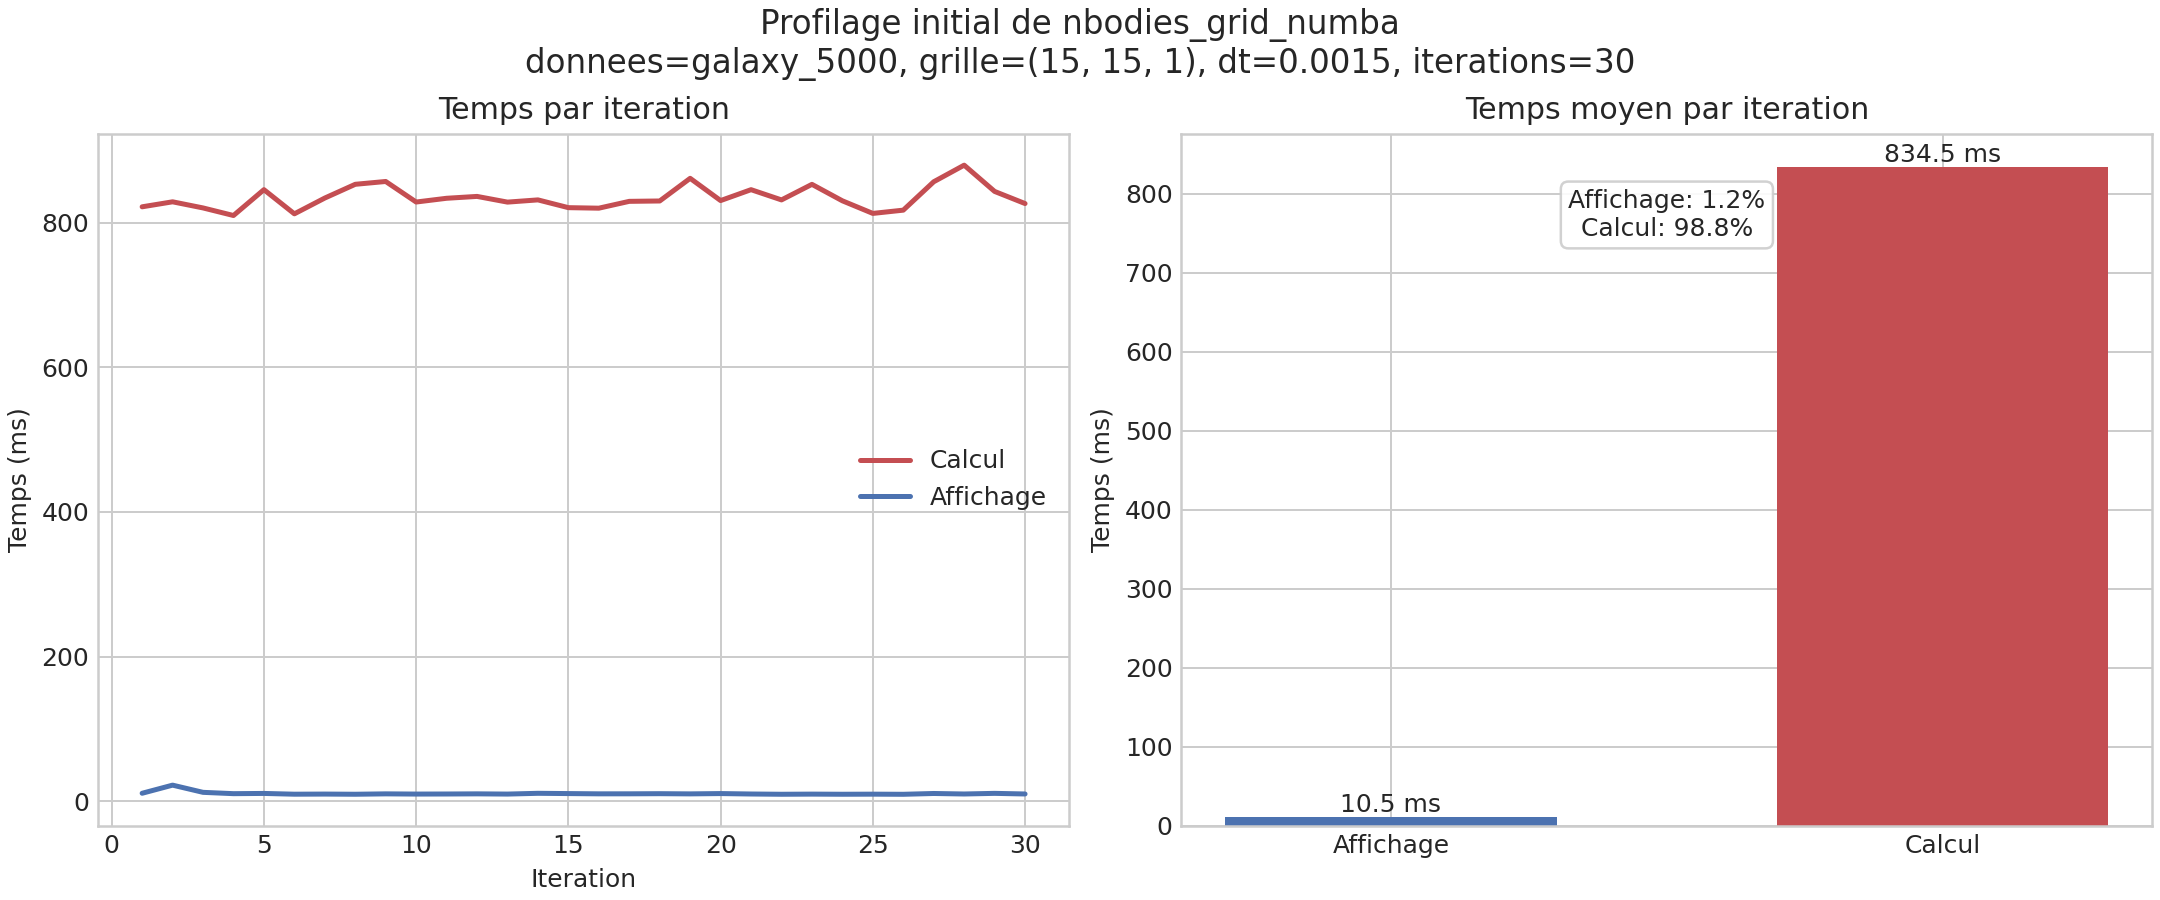
\includegraphics[width=\textwidth]{imgs/profilage_initial.png}
    \caption{Comparaison du temps moyen passé dans l'affichage et dans le calcul pour \texttt{nbodies\_grid\_numba.py}.}
\end{figure}


%---------------------------------------------------
% FIN DU RAPPORT.
%---------------------------------------------------

\end{document}
